\documentclass[11pt letter]{article}

\usepackage[utf8]{inputenc}
\usepackage[margin=0.7in]{geometry}
\usepackage{tikz}
\usepackage{nopageno}
\usepackage{graphicx}
\usepackage{amsmath}
\usepackage{setspace}
\onehalfspacing

\title{CS 381 - A8}
\author{Martin Mueller}
\date{Due: May $1^{st}$, 2020}

\begin{document}
\maketitle

\section{Problem 1}
Design a standard Turing machine that decides the language $A = \{0^{n^{2}}1 \ | \ n \ge 0\}$ in place.

\subsection{Formal Description}
\begin{itemize}
    \item $Q = \{q_0, q_1, ..., q_{10}, q_{accept}, q_{reject}\}$
    \item $\Sigma = \{0, 1\}$
    \item $\Gamma = \{\sqcup, 0, 1, x, y\}$
    \item $\delta$ is described by the state transition diagram.
    \item The start, accept, and reject states are $q_{0}$, $q_{accept}$, and $q_{reject}$ respectively.
\end{itemize}
\begin{center}
    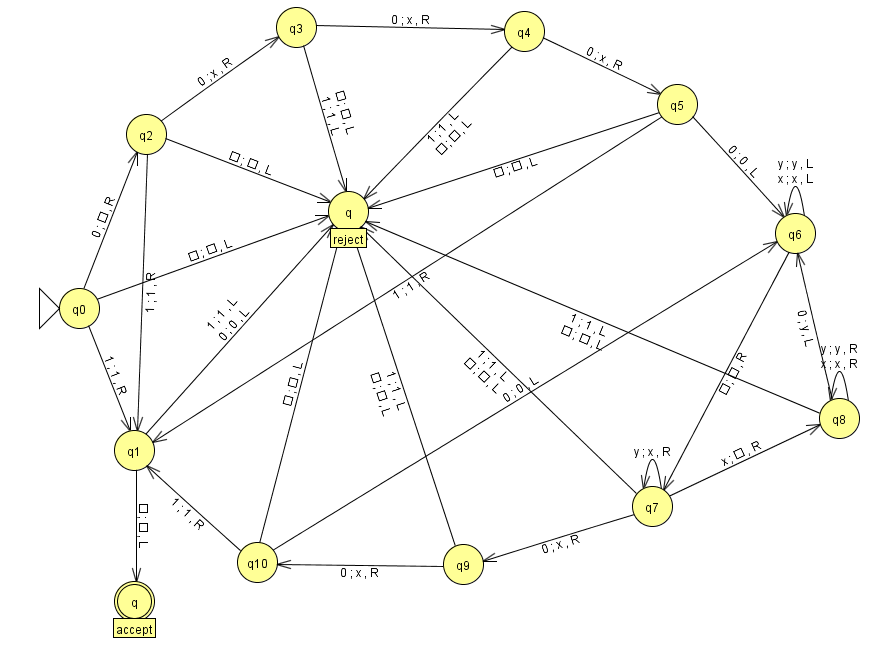
\includegraphics[scale=0.7]{TM.png}
\end{center}

\subsection{High-level Description}
\begin{enumerate}
    \item Reject if the Turing machine's head starts on a blank symbol.
    \item Accept if the input is just a single 1.
    \item Replace the first 0 with a blank symbol and move right.
    \item Reject if there is a blank symbol.
    \item Accept if only a single 1 is at the end of the input, but reject if other symbols follow the 1.
    \item Replace the next three 0's with $x$'s. Reject if the next three symbols are not 0's.
    \item Reject if the next symbol is a blank symbol.
    \item Repeat the following steps:
    \begin{enumerate}
        \item Accept if only a single 1 is at the end of the input, but reject if other symbols follow the 1.
        \item Replace the next several 0's with the entire preceding string of $x$'s, replace the old $x$'s with blank symbols, and replace the next two 0's with $x$'s. If this process is interrupted due to a lack of symbols or a symbol that is not 0, reject.
    \end{enumerate}
\end{enumerate}

\subsection{Justification}
This Turing machine utilizes a special property of square numbers: the square of a natural number $n$ is equal to the sum of the first $n$ odd natural numbers. For example:
    \begin{align*}
        1^2 &= 1 \\
        2^2 &= 1 + 3 \\
        3^2 &= 1 + 3 + 5 \\
        &\cdots
    \end{align*}
When the Turing machine copies over the preceding string of $x$'s and adds two additional $x$'s to the end, it's really adding the next odd natural number to the current sum. Each time the machine does this, it must check that there are enough 0's to do this with, and that only 0's exist in the next $n + 2$ spaces. Strings that interrupt this copy and add 2 section of the algorithm are rejected. At the end, the machine must simply check if the very last symbol is a 1. Any strings that do not fit this final pattern are immediately rejected.

\newpage

\section{Problem 2}
Assuming $A$ is an arbitrary language, prove that $A$ and the $\overline{A}$ are Turing-recognizable only if A is decidable.

\subsection{Proof}
A language $A$ is decidable if there exists a decider $M$ that accepts all $w \in A$. This means that $M$ must be able to definitively tell of a string is or is not in $A$. Such a machine would be able to recognize $A$ and $\overline{A}$ because it halts on both inputs in $A$ and inputs not in $A$.
\end{document}
